\section{Introduction}\label{section:intro}
The practice of experimental design entails specifying every detail of
running an experiment \cite{chaloner1995}: at its simplest form,
experimental design involves choosing a set of measurements to be
taken. For example, consider the process of searching for oil:
measuremnts are expensive and require digging holes in the ground, so
only a limited number of measuremnts can be taken, hence carefully
choosing measuremt locations is crucial.

Specifiyng the right set of measurements holds particular significance
when solving an \emph{inverse problem} --- i.e.~making inference of
the physical world utilizing a physical model a phenomenon of interest
\cite{tarantola2005,kaipio2005}. In an inverse problem, we seek to
infer physical quantities, based on observations and a model of the
physical world. Models are typically phrased in the language of
ordinary or partial differential equations.

Inverse problems are ubiquitous in science and engineering. For
example, in electrical impedance tomography (EIT) we seek to infer the
structure of the inside of a human body. Inference is conducted based
on observations of electrical current impedance measured at specific
electrode locations on the skin, leveraging known equations of
electric current flow \cite{horesh2010impedance}. Magnetic Resonance
Imaging (MRI) also entails solving an inverse problem. There,
radio-frequency pulses are sent through the human body in the presence
of a strong magnetic field. The response of one's body contents to
these radio-frequency pulses is measured, allowing a radiologist to
view the internals of a body in a noninvasive manner
\cite{horesh2008mri}. An inverse problem also arises in oil and gas
exploration. Acoustic waves are sent through "boreholes" --- deep
cylindrical wells drilled into the ground. Data of travel and return
times of the acoustic waves are recorded. Wave travel and return time
is influenced by the properties of the subsurface materials, such as
density, elasticity, and the presence of fluids or voids. Combining
travel data with a geophisical models of contents of the earth's crust
facilitates reconstructing and inferring the structure of the
subsurface in a process called \emph{borehole tomography}
\cite{horesh2008borehole}. Inverse problems also arise in many other
areas of seismology and geology \cite{rabinowitz1990, steinberg1995}
and medical imaging \cite{tarantola2005}. While in many inverse
problems the goal is to infer some parameter, in all of the above
examples and in the formulation we consider in this study, the goal is
to infer some \emph{function} over $ \Omega$, where (usually) \(\Omega
\subseteq \mathbb{R}^d, d=1,2,3\) is a spatial domain of interest.

\subsection{D-optimal Designs}\label{subsec:D}
In all of the examples of inverse problems we have seen, as well as in
many other applications, only a limited number of measurements are
allowed. For example, in borehole tomography, a measurement involves
drilling a deep well in the ground --- a very costly endeavor. Even in
a seemingly simpler application such as MRI, a patient cannot occupy
the MRI machine for too long, hence only a limited number of
measurements can be taken. Therefore, measurements should be chosen to
most benefit the user. Typically, a user will consider some utility,
called a \emph{design criterion} and take measurements that maximize
this utility. Two of the most widely recognized and extensively
studied design criteria are A- and D-optimality.

In this study, we focus on the Bayesian D-optimality
criterion. Bayesian D-optimality carries a simple and intuitive
meaning: measurements chosen according to the D-optimality criterion
maximize the expected Kullback-Liebler divergence from posterior to
prior \cite{chaloner1995, AlexanderianGloorGhattas14,
  CoverThomas91}. Utilizing KL divergence for quantifying distances
between distributions is standard practice and we will not motivate it
further here. For a discrete parameter $\param$ and data $\data$, the
KL divergence is defined as
\begin{equation}\label{eq:basic KL}
  D_{KL}\left (\Pr(\param|\data)||\Pr(\param)\right ) =  \sum_{\param} \log
  \frac{\Pr(\param|\data)}{\Pr(\param)} \Pr(\param|\data). 
\end{equation}
Of course, data $\data$ is not known before the experiment is
conducted, so we average over it to define the D-optimality criterion
as:
\begin{equation*}
  \mathbb{E}_{\data}\left [ D_{KL}\left (\Pr(\param|\data)||\Pr(\param)\right ) \right ]
\end{equation*}
We refer to a set of measuremnts that maximizes the D-optimality
criterion as a \emph{D-optimal design}.

For a linear model with Gaussian prior in finite dimensions, a
D-optimal design minimizes the determinant of the posterior covariance
\cite{chaloner1995}. In Section \ref{subsec:D optimal design} we give
a more general definition of the D-optimality criterion that applies
to arbitrary measures.

\subsection{A toy model: the 1D heat equation}\label{subsec:toy}
For concreteness, let us now consider a toy model of a physical process
for which we wish to solve an inverse problem: a partial differential
equation known as the \emph{heat equation} in one dimension (1D heat
equation henceforth, see details below). Readers less familiar with
partial differential equations can think of the following setup:
before us there is a perfectly insulated metal rod. At each point on
the rod the temperature is different and unknown, and we call this
temperature distribution the \emph{initial condition}. We wait for a
short time $T$ and let the heat dissipate a bit inside the rod. The
heat equation determines the heat distribution inside the rod at time
$t=T$.

The full time evolution of heat in the rod $\Omega=[0,1]$ is formally
described by the following three equations:
\begin{subequations}%\label{eq:heat equation}
  \begin{alignat}{2}
    u_t &= \Delta u &&\qquad \text{in } [0,1] \times [0,\infty), \label{eq:heat1}\\
    u &= 0 &&\qquad \text{on } \{0, 1\} \times [0,\infty), \label{eq:heat2}\\
    u &= u_0 &&\qquad \text{on }[0,1] \times \{0\}. \label{eq:heat3}
  \end{alignat}
\end{subequations}
As time passes, heat disspates across the rod as hotter regions,
e.g.~local maximas of the heat distribution, become cooler. This
behavior is captured by eq.~\eqref{eq:heat1}: the Laplacian at local
maxima is negative, so $u_t = \Delta u$ implies $u$ decreases at its
maximas, and the reverse happens at local minima. Eq.~\eqref{eq:heat2}
describes the \emph{boundary condition}, which dictates how heat
interacts with the outside world at the two edges of the rod
$\{0,1\}$. Specifically, eq.~\eqref{eq:heat2} implements an absorbing
boundary, i.e.~heat that interacts with the boundary is immediately
absorbed and disappears. This type of boundary condition is known as a
\emph{homogeneous Dirichlet boundary condition}. Eq.~\eqref{eq:heat3}
describes the \emph{initial conditions}, i.e.~the heat distribution
inside the rod at time $t=0$.

Solving the 1D heat equation is straightforward. Any initial heat
distribution $u_0\in L^2(\Omega)$ that satisfies the homogeneous
Dirichlet boundary condition is a linear combination of sines
$\ev_n(x) = \sin(2\pi n x)$. Now, note that $\ev_n$ are in fact
eigenvectors of the Laplace operator: $\Delta \ev_n = -(2\pi
n)^2\ev_n$. The linearity of the heat equation allows us to solve in
Fourier / frequency space. It is important to note that when solving
the heat equation we \emph{invert} the Laplace
operator. I.e.~eigenvalues of the linear operator associated with the
heat equation are $(2\pi n)^{-2}$.

In the \emph{inverse problem of the 1D heat equation}, our goal is to
infer the initial condition $u_0 = u(\cdot, 0)$ from observations of
the final condition $u(\cdot, T)$. However, we are not able to measure
$u(\cdot, T)$ at every point in the domain $\Omega$. Rather, we take
some number of temperature measurements on the rod once our waiting
time $T$ has passed and try to infer $u(\cdot, 0)$ from these
measurements.

The inverse problem of the 1D heat equation is difficult ("ill-posed")
since heat spreads in a diffusive manner and any roughness in the
initial condition is quickly smoothed, see Supplementary movies S1 and
S2. For ill-posed problems regularization is in order, and we
implement such regularization via a fully Bayesian formulation of the
inverse problem, see Section \ref{section:prelims} for details.


\subsection{Measurement Clusterization}
Surprisingly, A- and D-optimal designs for inverse problems have been
observed to yield remarkably similar measurements in certain cases
\cite{fedorov1996, nyberg2012, fedorov1997, Ucinski05,
  neitzel2019sparse}. This phenomenon is illustrated for our toy
inverse problem in Fig.~\ref{fig:clusterization illustration}, where
D-optimal measurement locations are shown for different numbers of
measurements. Notably, for six measurements, a D-optimal design yields
two sets of measurements that are identical. We refer to this
intriguing phenomenon as \emph{measurement clusterization}
\cite{Ucinski05}. We consider a design to be \emph{clustered} when two
or more of its constituent measurements are identical.

%% first: blue, second: red, third: green, fourth: black,
%% fifth:magenta
\begin{figure}
    \centering
    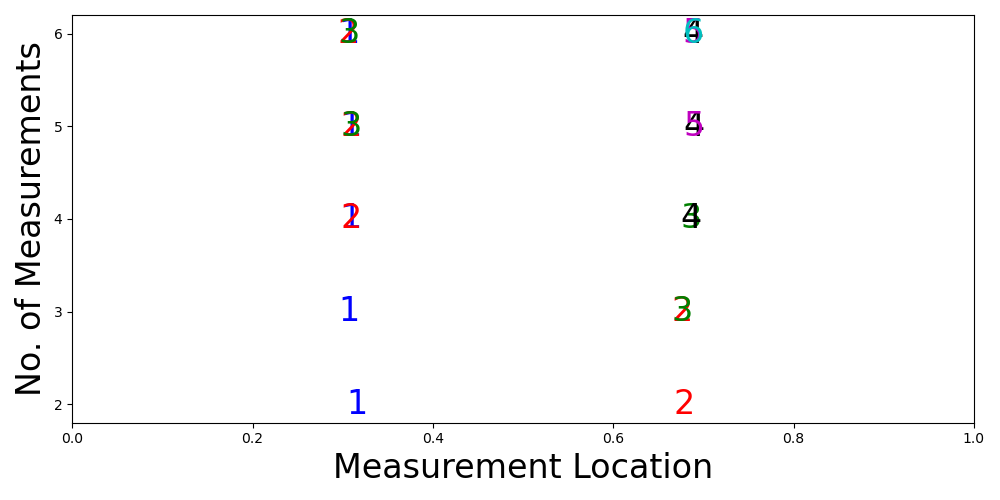
\includegraphics[height=0.5\textwidth]{dst_modelError0.png}
    \caption{Measurement clusterization for D-optimal designs for the
      inverse problem of the heat equation. Measurement locations were
      chosen according to the Bayesian D-optimality criterion of
      Theorem \ref{thm:d optimality}. Measurement locations are
      plotted over the computational domain \(\Omega = [0, 1]\)
      (x-axis), for varying numbers of measurements (y-axis). The
      colored numbers are measurement indices, plotted for visual
      clarity. Measurement clusterization already occurs for three
      measurements: the second measurement (red) is overlaid on the
      third (green). For five measurements, first (blue) and second
      (red) measurements are clustered, as well as the fourth (black)
      and the fifth (magenta).}
  \label{fig:clusterization illustration}
\end{figure}


Clusterization should not be confused with either repetition nor with
replication, which are commonly viewed as beneficial and even
necessary aspects of an optimal design \cite{morris, fisher
  schafer2001replication}. For example, in his famous milk and tea
experiment, \cite[Section 11]{fisher} suggested that repetition is a
"way of enlarging the experiment and, thereby, increasing its
sensitiveness". In another example, \cite{fay2000rainfall} measured
the effect of rainfall on grass growth in plots of land. The
experiment involved fifteen "rainfall manipulation shelters", where
"Four rainfall manipulation treatments (three replicates) then were
assigned to 12 of the plots". It seems reasonable the researchers
replicate the phenomenon they are trying to study. Clusterization is
different: a clustered design in the rainfall experiment would imply
the researchers should take a repeated measurement \emph{on the same
plot}, at the expense of measuring grass growth in other plots. In
sharp contrast to repetition and replication, clusterization is highly
nonintuitive and we will see that its origins run considerably deeper.


Researchers of inverse problems widely agree that measurement
clusterization is undesirable
\cite{fedorovDesignSpatialExperiments1996, nyberg2012, fedorov1997,
  Ucinski05, neitzel2019sparse}, prompting the exploration of various
remedies to address this issue. One approach involves merging close
measurements \cite{fedorov1997}; however, this strategy merely
overlooks the phenomenon of measurement clusterization. An alternative
solution lies in \emph{clusterization-free design}s, where measurement
locations are deliberately chosen to be distant from one another. This
can be achieved by imposing distance constraints between measurements
or by introducing correlated errors that account for both observation
error and model misspecification \cite{Ucinski05}. For instance, in
the context of time-series analysis for pharmacokinetic experiments,
measurement clusterization can be mitigated by incorporating the
modeling of auto-correlation time within the noise terms
\cite{nyberg2012}.


In spatial problems involving choice of measurements within a domain
\(\Omega \subseteq \mathbb{R}^d, d=1,2,3\), many researchers
circumvent the problem of measurement clusterization by choosing
measurements from a coarse grid in \(\Omega\) \cite{koval2020,
  alexanderian2021, attia2022, alexanderian2014, alexanderian2016,
  alexanderian2018efficient, brunton2016}. This approach incurs a
significant computational cost as it requires solving a difficult
combinatorial optimization problem for measurement locations over a
discrete set. The combinatorial optimization problem is usually
relaxed by first assigning optimal measurement weights in
\(\mathbb{R}_+\) to the potential measurement locations. Some
researchers incorporate a sparsifying \(\ell_1\) penalty term into the
design criterion, which is subsequently thresholded to achieve the
desired binary design over the coarse grid
\cite{horesh2008borehole}. Others progressively relax the \(\ell_1\)
penalty to an \(\ell_0\) penalty via a continuation method
\cite{alexanderian2016, alexanderian2014}. Others cast the problem of
finding optimal measurement weights as a stochastic optimization
problem \cite{attia2022stochastic}. All of the aforementioned methods
may indeed find a binary optimal design restricted to a given coarse
grid. However, none addresses one fundamental issue: the restriction
of measurement locations to a coarse grid in \(\Omega\) fundamentally
changes the optimal design problem and thus results in a sub-optimal
design.

Avoiding measurement clusterization is a pragmatic approach:
intuitively, researchers recognize that measurement clusterization is
undesirable, even though the underlying reasons may not be fully
clear. Consequently, they strive to prevent it and devise various
methodologies to avoid it. Yet each and every one of these
methodologies achieves its objective by imposing restrictions on
measurement locations, thereby fundamentally altering the optimal
design problem. To the best of my knowledge, no previous study has
tried to address some seemingly simple yet fundamental questions:
%
Why does imposing correlations between observations alleviate
measurement clusterization?
%
Is measurement clusterization a generic phenomenon? 
%
And, most importantly: Why does measurement clusterization occur?
%
%Should we aim to avoid measurement clusterization?
%
%Is it possible to substitute an optimal clustered design with an
%equally optimal non-clustered design?
%Can an optimal clustered design be relpaced with an equally optimal
%non-clustered design?


\subsection{Contribution}
The primary objective of this study is to provide a deep understanding
of measurement clusterization by addressing the aforementioned
questions. Our focus centers around investigating the Bayesian
D-optimality criterion. We conduct an analysis of Bayesian D-optimal
designs within the context of linear inverse problems over Hilbert
spaces and study two inverse problems: (a) In Sections
\ref{section:prelim} and \ref{section:D and grad} we propose a novel
relaxed model for an inverse problem where D-optimality maintains
analytical tractability. In this model D-optimal designs are
identified via Lagrange multipliers. This analytical framework
facilitates the exploration of the questions posed at the end of the
previous paragraph. (b) we also study the inverse problem of the 1D
heat equation (see Section \ref{subsec:toy} above). Investigating both
inverse problems allows us to answer the questions posed in the
previous section:

\begin{enumerate}
\item \label{q:generic} \textbf{Is measurement clusterization a
  generic phenomenon?}
  %\subsection{An answer for Question \ref{q:generic}: Genericity of measurement clusterization}
  %% Computer implementation of Lemma \ref{thm:char} for the inverse
  %% problem outlined in Section \ref{section:how} also generates \(\obs\)
  %% as a solution to the D-optimal design problem.  Furthermore,
  We give two complementing answers to this question. First, from a
  theoretical perspective, we show that clusterization barely depends
  on the specifics of the prior, so long as it is Gaussian. We show
  that the structure of the decay of the eigenvalues of the
  pushforward prior covariance determine clusterization. The decay of
  these eigenvalues depends mostly on how ill-posed the problem at
  hand is and does not depend much on the prior. See Section
  \ref{section:vanishing} --- particularly, Theorem \ref{thm:char} and
  the discussion following it. We also show results of numerical
  experiments, where simulations of our model give rise to D-optimal
  designs that exhibit clusterization with very high probability in
  Section \ref{subsec:lemma sims}. Thus, given the genericity of our
  model, we expect measurement clusterization to be a generic and
  ubiquitous phenomenon.

\item \label{q:mitigate} \textbf{Why does imposing correlations
  between observations alleviate measurement clusterization?} In
  Section \ref{section:non vanishing}, we rigorously demonstrate the
  role of model error in mitigating clusterization, thereby
  corroborating earlier observations made by various
  researchers. Specifically, our proof shows that identical
  measurements result in no gain in design criterion in when
  observation error tends to zero. Moreover, in Section
  \ref{subsec:corr errors sims}, we show that adding to the inverse
  problem of the 1D heat equation an error term corresponding to
  correlations between measurements mitigates clusterization.

\item \label{q:why} \textbf{Why does measurement clusterization
  occur?} In Section \ref{subsec:why} we give a compelling answer to
  this question by transporting insights we gain from our analytically
  tractable relaxed model to the inverse problem of the 1D heat
  equation. Our analysis reveals that a D-optimal design focuses on a
  select set of prior eigenvectors, specifically those with the
  largest eigenvalues in the prior covariance spectrum. In practical
  scenarios, the number of locations where (a) all relevant prior
  eigenvectors are significantly large, and (b) other eigenvectors are
  close to zero, is limited. Consequently, the clusterization of
  measurements arises as a natural consequence of the pigeonhole
  principle, as there are more measurements available than there are
  locations satisfying conditions (a) and (b). See Fig~\ref{fig:why}.


  %% In Section \ref{section:vanishing}, we provide an insightful
  %% explanation for the optimality of clustered designs when no model
  %% error is present. We demonstrate that for our model, a D-optimal
  %% design measures only a small subset of prior eigenvectors, which are
  %% the prior eigenvectors with largest power spectrum. In real-life
  %% problems there are limited number of locations where: (a) the
  %% relevant prior eigenvectors are large, and other prior eigenvectors
  %% with large power in the prior spectrum are zero. Then measurement
  %% clusterization is a result of the pigeonhole principle, where there
  %% are more measurements than measurement locations satisfying (a) and
  %% (b).

  %% We conjecture that the prevalence of measurement clusterization
  %% arises due to the ease of discovering clustered designs.


%% \item \label{q:avoid} \textbf{Should we aim to avoid measurement
%%   clusterization?} Based on the analysis conducted in this study, we
%%   did not find any compelling reason to explicitly avoid optimal
%%   clustered designs.

%% \item \label{q:replace} \textbf{Is it possible to substitute an
%%   optimal clustered design with an equally optimal non-clustered
%%   design?} In Section \ref{section:vanishing}, we answer this question
%%   in the affirmative, although we show that numerical experiments
%%   conducted using our model indicate a strong preference for clustered
%%   designs.
\end{enumerate}

\subsubsection{Implications}
Our answer to Question \ref{q:generic} implies that encountering
clusterization should be expected in many different problems across
many different scientific fields. Thus, researchers that encounter
clusterization should not be surprised or wary. In Our answer to
Question \ref{q:why}, we explain what our view of the cause of
clusterization. As it appears, the cause is generic (see Question
\ref{q:why} above): a D-optimal design reduces uncertainty for a
select set of prior covariance eigenvectors --- those with the most
prior uncertainty, i.e.~those the practitioner cares about the most!
Consequently, practitioners should not try to avoid measurement
clusterization. Rather, practitioners should take repeated
measurements (e.g.~in MRI and borehole tomography), increase apparatus
sensitivity (e.g.~in EIT), or take consecutive measurements (e.g.~in
the 1D heat equation). Overall, we show that measurement
clusterization is a natural and (almost) inevitable part of Bayesian
D-optimal designs.

One interesting implication of the analysis presented here is that
clusterization can be expected once the number of measurements exceeds
the number of relevant eigenvectors. Since leading eigenvectors
typically correspond to slow variations in space and/or time,
clusterization could be used to estimate the number of relevant
degrees of freedom, and even to reduce the complexity of a
computational model, e.g.~by dropping discretization points.

It is important to note that we do not view measurement clusterization
as undesirable, nor do we believe it should be avoided at
all. Clusterization is a peculiar phenomenon and it is perfectly
reasonable for someone to argue against the D-optimality criterion
based on the fact that it results in clustered designs. We have seen,
however that there is perfectly reasonable explanation for
clusterization, i.e.~that clusterization arises when we seek a
designWe have shown that clusterization is an innevitable conseqeunce
of having a problem with modes of higher uncertainty than
others. Clusterization manifests the true underlying objective




\subsubsection{Other Contributions}
In Theorem \ref{thm:char}, we also show that D-optimal designs are
best understood in the sapce of \emph{observations}, see Section
\ref{section:vanishing} for a precise statement. This is in accordance
with previous work by \cite{koval2020}, who showed that A-optimal
designs are best constructed in the space of observations.

In the process of proving Theorem \ref{thm:char} we prove and
generalize several lemmas. Among those, is Lemma \ref{lemma:free},
which is (to the the best of my knowledge) novel: We decompose a
symmetric positive definite matrix \(M \in \mathbb{R}^{k \times k}\)
with \(\ttr M = m \in \mathbb{N}\) as \(M = AA^t\), where \(A\in
\mathbb{R}^{k \times m}\) has unit norm columns.

%% Finally, in Lemma \ref{lemma:lax} we generalize a lemma for
%% calculating \(\frac{\der}{\der t} \log \det (I + X(t))\), where
%% \(X(t)\)is an operator valued function \cite{Lax07}.

%% Finally, we must stress that we do not advocate any particular
%% solution to clusterization. We do not suggest that clustered designs
%% should be abandoned, nor do we support the use of clustered designs in
%% any circumstances. Our goal is to investigate an intriguing phenomenon
%% of clusterization and seek a deeper understanding for it. Different
%% researchers in different disciplines have differenot viewed as a problem. For
%% example, \cite{lozan} suggest in the introduction section that
%% repeated measurements are necessary. Our results align with that
%% common wisdom and settle the seemed contradiction.


\subsection{Limitations}\label{subsec:limitations}
The main limitation of this study is that our generic model does not
correspond to any specific real-life problem. Specifically, in its
current form, our model does not allow point evaluations, see the
Discussion for a deeper analysis of this subject. Our model is generic
enough to be analytically tractable, but one may argue our model is
too far removed from any real application. To these claims I would
answer that scientists have a long history of studying models that are
bare-bones simplifications of real systems, e.g. the Ising model
\cite{cipra1987}, the Lorenz system \cite{brin}, the Lotka-Volterra
equations \cite{logan2006}, the Carnot engine \cite{kardar2007}, and
many others.
